
\documentclass[a4paper, 12pt, titlepage]{article}
\usepackage{graphicx}

\usepackage[utf8]{inputenc}
\usepackage[T1]{fontenc}

\usepackage{times}
\usepackage[english,swedish]{babel}
\usepackage{graphicx}

\usepackage{fancyhdr}

%----------------------------------------------------------------------------------------
%	TITLE
%----------------------------------------------------------------------------------------

\title{Lab 1 TNM031}
\author{Carl Englund \\ caren083}


\pagestyle{empty}
\thispagestyle{empty}

\begin{document}

\maketitle % Print the title section

\section{The Basic HTTP GET/response interaction}
	\textbf{1.} Both the server and client is using version 1.1
	\\\textbf{2.} It can only accept HTML.
	\\\textbf{3.} My ipadress is 130.236.124.35. The adress of the website is 128.119.245.12.
	\\\textbf{4.} The status code returned from the website is 200. This means that everything is OK.
	\\\textbf{5.} Last Modified: Tue 01 Sep 2015.
	\\\textbf{6.} 552 bytes.


\section{The HTTP CONDITIONAL GET/response interaction}

	\textbf{7.} No, there's nothing there at the moment.
	\\\textbf{8.} Yes. One can see it in the Line-based text data field.
	\\\textbf{9.} Yes. The date is since the last time i requested the site.
	\\\textbf{10.} The status code returned is 304, which says that the file has not been modified. Since this happened the server does not return anything and instead the browser uses my cached version of the website. A very nice way to save time and bandwith.

\section{Retrieving Long Documents}

	\textbf{11.} One HTTP GET request were sent by my browser.
	\\\textbf{12.} Four TCP segments were needed.
	\\\textbf{13.} 200 Response phrase: OK
	
\section{HTML Documents with Embedded Objects}

	\textbf{14.} Four GET requests were sent see figure \ref{figure}. 
		\\One to retrieve the HTML file from \emph{webstaff.itn.liu.se}.
		\\One to retrieve the gif image from \emph{www.liu.se}.
		\\One to retrieve the image pi.jpg from \emph{www.ox.ac.uk}. 
		\\And the last one to fetch the favicon for the site from \emph{webstaff.itn.liu.se}. 
	\\\textbf{15.} They are done serially according to Wireshark. This can be seen in figure \ref{figure}. Since the times for the different GET-requests differs some it can be determined that it's performed serially.

\section{HTTP Authentication}
	\textbf{16.} Status code 401. Authorization required.
	\\\textbf{17.} The new field is an authorization field. I can see the credentials i just entered for the website which is a bit scary since they are not encrypted at all.

\begin{figure}[p]
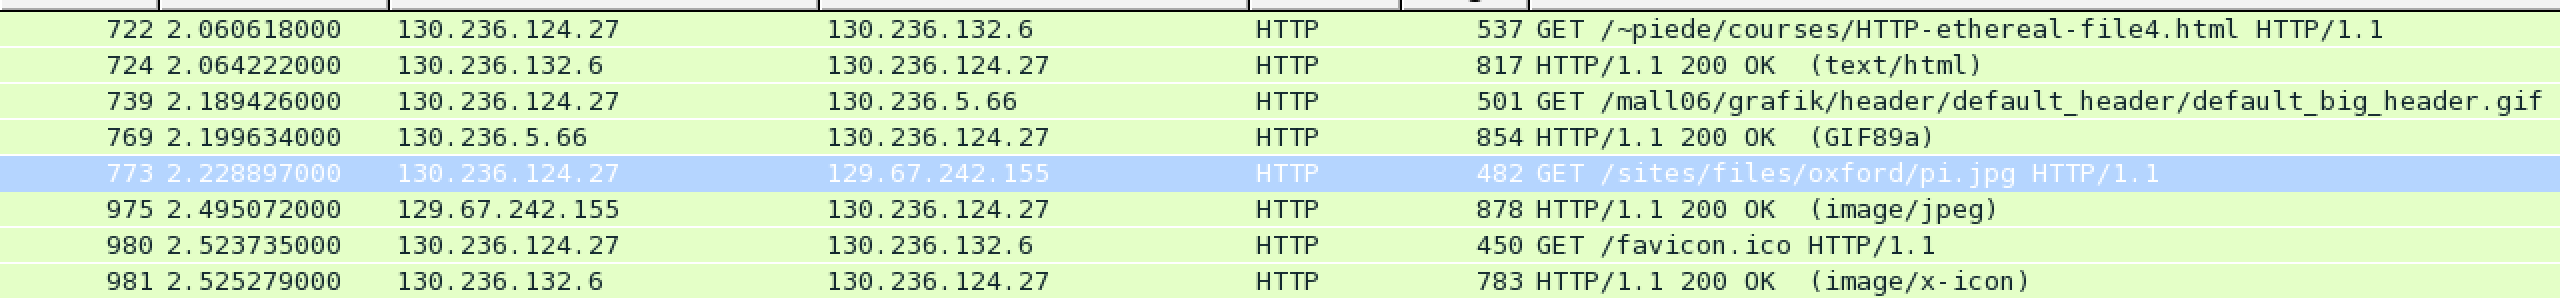
\includegraphics[angle=90, scale=0.5]{pic}
\caption{Wireshark response to question 14}
\label{figure}
\end{figure}
\end{document}